\documentclass[aps,prl,reprint,10pt,amsmath,amssymb,superscriptaddress,a4paper, floatfix]{revtex4-2}
\usepackage{graphicx, booktabs} % Graphics package
\usepackage{epstopdf, float} % Convert EPS to PDF
\usepackage{dcolumn} % Double column package
\usepackage{amsmath,amsfonts,amsthm} % Math packages
\usepackage[hidelinks=True]{hyperref} % Hyperref package
\usepackage[margin=2cm]{geometry} % Sets 2cm margins
\usepackage{datetime} % Package for automatic date & time
\usepackage{lipsum} % Inserts dummy latin text into template -- Can remove from final submission
\graphicspath{{Diagrams/}} % Sets path for graphics, CHANGE WHEN WORKING ON MACOS
%\setcitestyle{authoryear,round}
\begin{document}
\title{PHYS2113: Coupled Pendula}

\author{S.J Shelton (z5359712)}
\affiliation{Cohort B - Friday 2-5 class}
\affiliation{Word count: c. 3000 words}
\date{\currenttime~\today}

\begin{abstract}

In this paper, Newtonian mechanics and the small angle approximation are used to derive equations of motion for a system of coupled pendula. This model is found unable to make precise quantitative predictions, and an improved model using an experimentally determined $\omega_n$ (natural frequency) is developed. Alternate models using numerical methods are explored.

\end{abstract}

\maketitle
% You start your main text after here.

\section{Introduction}
A set of coupled pendula consists of two otherwise independent pendulums linked by some mechanism, in this case a spring. Coupled pendula are a natural progression from the simple pendulum, and the mathematics behind them represents a clear step up, requiring a working knowledge of differential equations and some rotational dynamics.

In order to make the differential equations for the coupled pendulum analytic and easily solvable, we will use a Taylor series approximation. We are only interested in the first order approximations, that is, $\sin x = x$ and $\cos x = 1$.

We begin by finding our equation for the torque in terms of angular acceleration. Recall that, for a point mass a distance out from a rotational axis (a pendulum is an example of this), $I = mR^2$.

\[\tau = I \ddot{\phi}_1 = L F_g \sin(\phi_1) + \ell F_s \cos(\phi_1) \]

\begin{equation}
\label{eqn1}
m L^2 \ddot{\phi_1} = -Lmg \sin \left( \phi_1 \right) - \ell k \Delta x \cos \left( \phi_1 \right)
\end{equation}

Recall the expression for the natural frequency of a pendulum from first year, note that this expression itself required the small angle approximation to be derived.

\begin{equation}
    \omega_n = \sqrt{\frac{g}{L}}
\end{equation}

\begin{figure}[t]
    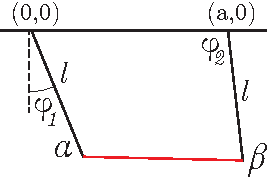
\includegraphics[width = 7 cm]{Asset 5.pdf}
    \caption{Vector space to find $\Delta x$}
    \label{fig:vectorspace1}
\end{figure}

Now we must find an expression for $\Delta x$. First consider the Vector space from figure \ref{fig:vectorspace1}.

\[
\vec{\alpha} \ = \begin{pmatrix} 0 + \ell \sin \phi_1 \\ 0 + \ell \cos \phi_1 \end{pmatrix}, \qquad
\vec{\beta} \ = \begin{pmatrix} a + \ell \sin \phi_2 \\ 0 + \ell \cos \phi_2 \end{pmatrix}\
\]\[
\therefore \overrightarrow{\alpha \beta} = \begin{pmatrix} \ell \sin \phi_2 + a - \ell \sin \phi_1 \\ \ell \cos \phi_2 - \ell \sin \phi_1 \end{pmatrix}
\]\[
|\overrightarrow{\alpha \beta}| = \begin{pmatrix}  \ell \phi_2 - \ell \phi_2 + a \\  \ell \phi_2 - \ell \phi_1 \end{pmatrix} = \begin{pmatrix}  \ell ( \phi_2 - \phi_1 ) + a \\  0 \end{pmatrix}
\] \begin{equation}
\therefore \Delta x = |\overrightarrow{\alpha \beta}| - a = \ell \left(\phi_2 - \phi_1\right)
\label{eqn:2}
\end{equation}

We have already applied the small angle approximation to get \ref{eqn:2}. We apply the same approximation to equation \ref{eqn1}, and substitute in the expression for $\Delta x$ from \ref{eqn:2} to derive:

\begin{equation}
   mL^2 \ddot{\phi}_1 = - L m g \phi_1  - \ell^2 k \left( \phi_2 - \phi_1 \right)
\end{equation}

With some rearrangement, and by recognising the symmetry of the system (spring force acts in the opposite direction for the other pendulum), we find:

\begin{equation}
\ddot{\phi}_1 + {\omega_n}^2 \phi_1 = - \left( \frac{\ell}{L} \sqrt{\frac{k}{m}} \right)^2  \left(\phi_2 -  \phi_1\right)
\end{equation} \begin{equation}
\ddot{\phi}_2 + {\omega_n}^2 \phi_2 = \left( \frac{\ell}{L} \sqrt{\frac{k}{m}} \right)^2  \left(\phi_2 -  \phi_1\right) 
\end{equation}

We now have a system of coupled, homogeneous, second order linear differential equations.

We are interested in three solutions corresponding to three distinct initial conditions. These are the in-phase mode, where the pendulums start at the same non-zero angles; the out-of-phase mode, where the pendula start with equal but opposite angles; and the beat mode, where one of the pendula starts at rest.

\pagebreak

\begin{widetext}
\begin{figure*}[t]
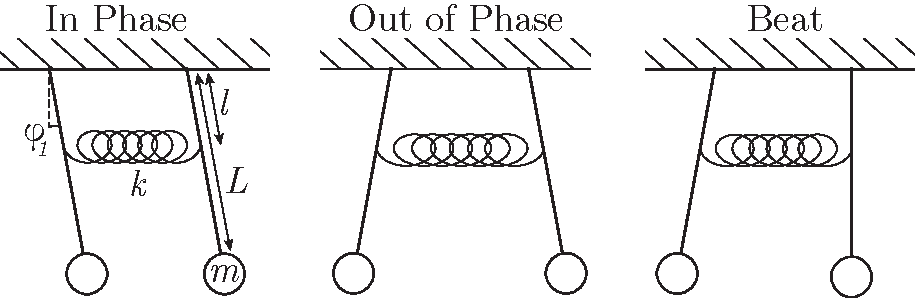
\includegraphics[width = 16 cm]{Modes and Variables Diagram.pdf}
\caption{A Basic Overview of a Coupled Pendula System, with different vibrational modes and required variables shown.}
\label{fig:modesandvariables}
\end{figure*}

We are given solutions in the experimental notes \cite{notes}. They are, for the in and out of phase modes respectively:

\begin{equation}
\phi_1 \left( t \right) = \phi_2 \left( t \right) = \phi_\text{max} \cos \left( \omega_n t \right)
\end{equation} \begin{equation}
\phi_1 \left( t \right) = - \phi_2 \left( t \right) = \phi_\text{max} \cos \left( \sqrt{\omega_n^2 + \frac{2 \ell^2 k}{L^2 m}} t \right)
\end{equation}

The beat vibrational mode is significantly more complex, but it is important to note that, by the nature of linear ODEs (and the fact that the in and out-of-phase modes make up the basis for equation), the beat mode is a linear superposition of the other state. We are given:

\begin{eqnarray}
\label{eqn2} \phi_1 = \phi_\text{max} \cos \left( \frac{\sqrt{\omega_{n}^{2}+\frac{2 l^{2} k}{L^{2} m}} - \omega_n}{2} t \right)\cos \left( \frac{\sqrt{\omega_{n}^{2}+\frac{2 l^{2} k}{L^{2} m}} + \omega_n}{2} t \right) \\
\label{eqn3} \phi_2 = - \phi_\text{max} \sin \left( \frac{\sqrt{\omega_{n}^{2}+\frac{2 l^{2} k}{L^{2} m}} - \omega_n}{2} t \right)\sin \left( \frac{\sqrt{\omega_{n}^{2}+\frac{2 l^{2} k}{L^{2} m}} + \omega_n}{2} t \right) 
\end{eqnarray}
\end{widetext}

We can quite easily perform a Fourier decomposition by inspection of the first two modes\cite{note1}:

\begin{equation}
\phi_1 \left(\omega\right) = \phi_2 \left(\omega\right) = \delta \left(\omega - \omega_n\right)
\end{equation} \begin{equation}
\phi_1 \left( \omega \right) = \phi_2 \left( \omega \right) = \delta \left(\omega - \sqrt{\omega_n^2 + \frac{2 \ell^2 k}{L^2 m}} \right)
\end{equation}

For brevity, let us define:
\begin{equation} \omega'_\ell = \sqrt{\omega_n^2 + \frac{2 \ell^2 k}{L^2 m}  } \label{omega'}  \end{equation}

For the third mode, we know it must be some linear superposition of the base states, it follows that it’s Fourier decomposition should be a combination of that of the basis states, i.e.:

\begin{equation}
\phi_1 \left( \omega \right) = \phi_2 \left( \omega \right) = \delta \left(\omega - \omega'  \right) + \delta \left(\omega - \omega_n\right)
\end{equation}

To surmise the model: The modes of interest can be modelled analytically by using the small angle approximation and solving a system of second order ODEs. In order to verify the model experimentally, the Fourier decompositions of the model and experimental data must be compared. The model's values for these are as follows:

%it is necessary to compare Fourier decompositions. The theoretical expected value for these are as follows:

\vspace*{12px}

\noindent \textbf{ i) In-Phase:}  In-Phase Mode 

\[ \phi_1 \left( \omega \right) = \phi_2 \left( \omega \right) = \delta \left(\omega - \omega_n\right) \]

\noindent \textbf{ ii) Out-of-Phase:} Out-of-Phase Mode 

\[ \phi_1 \left( \omega \right) = \phi_2 \left( \omega \right) = \delta \left(\omega - \sqrt{\omega_n^2 + \frac{2 \ell^2 k}{L^2 m}}  \right) \]
    
\noindent \textbf{ iii) Beat:} Beat Mode

\[ \phi_1 \left( \omega \right) = \phi_2 \left( \omega \right) = \delta \left(\omega - \sqrt{\omega_n^2 + \frac{2 \ell^2 k}{L^2 m}}  \right) + \delta \left(\omega - \omega_n\right) \]

\section{Aim}

To conduct an experiment to validate our theoretical model for a system of coupled pendula, considering all three vibrational modes and their dependancies on specific variables. That is, to make both quantitative and qualitative comparisons between the model and experimental reality.

If possible we should aim to explore where the model brakes down -- specifically in the context of the assumptions that have been made -- and, if possible, to suggest improvements or fixes to increase the usefulness of the model.

%We will conduct an experiment to verify the relationships we have just derived for the coupled pendulum. We should consider all three vibrational modes, as well as a non-coupled pendulum, and consider the dependence of the composite modes with respect to variables $k$ and $\ell$.

%Our aim is to validate our theoretical model: We want to know both how accurate it is purely numerically as well as how accurate it is at reflecting the relationships between variables.

%We also need to be aware of our assumptions, and where and why our model works or breaks down, and possibly derive or suggest improvements while critically evaluating our model both quantitatively and qualitatively.

\section{Method}

\begin{figure}
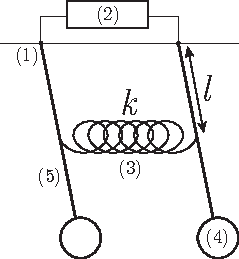
\includegraphics[width = 8 cm]{Method Diagram.pdf}
\label{fig:setup}
\caption{The Experimental Setup}
\end{figure}

The experimental apparatus in figure \ref{fig:setup} was set up with a pendulum of length $L = 1$ m (5), a mass $m = 1$ kg (4), and a spring that connects the pendulum with spring constant $k = 1$ N/m (3), located $\ell$ m from the pivot. The pivot itself (1) is a potentiometer, which records a voltage that corresponds to the angular displacement of the mass. This information is sent to a computer (2) for processing and Fourier transformation.

For data collection, it is important to recognise that because of the mechanics of the Fourier transform, longer periods of observation will yield significantly less errors, increasing experimental precision.

The following experimental trials were carried out for the maximum time available (usually between 700 and 1200 seconds). The precise time interval is not important, although keeping the trails of comparable general length is beneficial for the data analysis. 700 and 600 second trials is fine, but 30 and 1200 seconds is not.

\begin{table}[]
\begin{tabular}{@{}lllll@{}}
\toprule
             & $\ell = 0.2$       & $\ell = 0.4$      & $\ell = 0.6$      &  \\ \midrule
Uncoupled    & \multicolumn{3}{l}{3 Trials per   pendulum} &  \\
In-Phase     & 1 Trial       & 1 Trial      & 1 Trial      &  \\
Out-of-Phase & 3 Trials      & 3 Trials     & 3 Trials     &  \\
Beat         & 3 Trials      & 3 Trials     & 3 Trials     &  \\ \bottomrule
\end{tabular}
\caption{Experimental Trials Carried Out}
\end{table}

Multiple trials are not required for the In-Phase mode because we don’t expect results to vary with $\ell$. If any variance is observed during the conduct of the experiment, more investigation is required. The uncoupled trials establish the independence of the pendula.

For error analysis, Gaussians were fitted to the Fourier transforms of collected data. Standard deviations were extracted and pooled from trials, and a confidence interval ($2 \sigma$) extracted. \textsc{Mathematica}’s \texttt{Around} function was used for error propagation.

Additionally, values for $k$ were determined experimentally (with uncertainty) though a linear regression of deformation under a varied weight force.

\section{Results \& Analysis}

The linear regression for the spring constants yielded the following values with uncertainties. 

The first two modes used a different spring (and thus, different $k$) than the Beat mode.

\begin{table}[h]
\begin{tabular}{@{}lllll@{}}
\toprule
             & $k$ (kg / s$^2$)       & $U$ ( $95 \%$ CI)  \\ \midrule
In/Out of Phase         & $3.11$      & $0.22$     &   \\
Beat         & $2.99$      & $0.29$     & \\ \bottomrule
\end{tabular}
\caption{Spring Constants from Linear Regression}
\end{table}

We can now make predictions for experimental frequencies. $\omega_n$ is the natural frequency, $\omega'_\ell$ is from \ref{omega'} evaluated at a certain $\ell$ using the first spring constant, and $\omega''_\ell$ is the same but with the latter spring constant (for the beat).

\begin{table}[h]
\begin{tabular}{@{}lllll@{}}
\toprule
                    & Rads$/$s    & U ($95 \%$ CI)  & \\ \midrule
$\omega_n$          & $3.13$      & $0.00$          & \\ 
$\omega'_{0.2}$     & $3.17$      & $0.00$          & \\ 
$\omega'_{0.4}$     & $3.29$      & $0.01$          & \\
$\omega'_{0.6}$     & $3.47$      & $0.02$          & \\ 
$\omega''_{0.2}$    & $3.17$      & $0.00$          & \\ 
$\omega''_{0.4}$    & $3.28$      & $0.01$          & \\
$\omega''_{0.6}$    & $3.46$      & $0.03$          & \\ \bottomrule
\end{tabular}
\caption{Expected Fourier Values with Uncertainties}
\end{table}
    
Now we can analyse the data from the individual experiments with these expectations.

\subsection*{Uncoupled Pendulum}

The goal of this experiment specifically is to establish the independence of the pendulum. We will take pooled means and standard deviations from the left and right pendulum, compare them and, if appropriate, combine them.

\begin{figure}[H]
    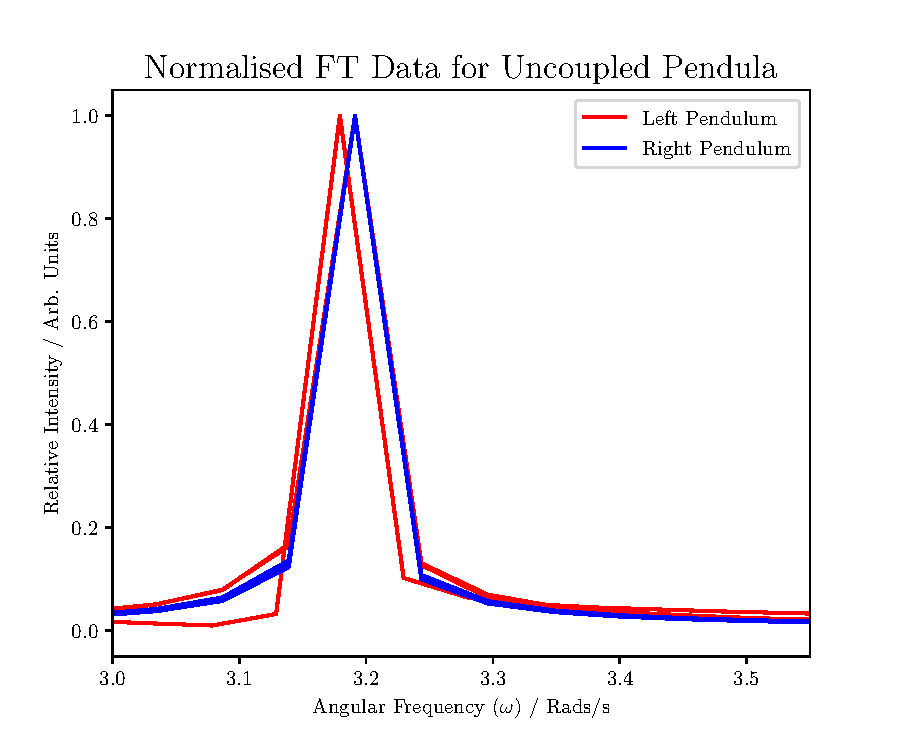
\includegraphics[width = 8 cm]{Normalised Independant FT.pdf}
    \caption{Independant Pendula Fourier Transform Data}
    \label{fig:independent}
\end{figure}

\begin{table}[h]
    \begin{tabular}{@{}lllll@{}}
    \toprule
                      & Rads$/$s    & U ($95 \%$ CI)  & \\ \midrule
    Left Pendulum     & $3.19$      & $0.05$          & \\ 
    Right Pendulum    & $3.19$      & $0.05$          & \\ 
    Pooled Pendula    & $3.19$      & $0.05$          & \\
    Model             & $3.13$      & $0.00$          & \\ \bottomrule
    \end{tabular}
    \caption{Uncoupled Pendula Data Comparison}
\end{table}

An $F$ test can quite easily determine that there is no evidence to support any variation between these two pendula, they behave identically and with no mutual dependency.

It is now important to note that our model has not precisely predicting the angular frequency. If we use this result, $\omega = 3.19 \pm 0.05$, as an experimentally determined value for $\omega_n$, we can refine our model by using this experimental value in place of our predicted $ \omega_n = \sqrt{g}$.

For brevity, we will call this revised model $\textnormal{model}'$.

\begin{table}[h]
    \begin{tabular}{@{}lllll@{}}
    \toprule
                        & Rads$/$s    & U ($95 \%$ CI)  & \\ \midrule
    $\omega_n$          & $3.19$      & $0.05$          & \\ 
    $\omega'_{0.2}$     & $3.23$      & $0.05$          & \\ 
    $\omega'_{0.4}$     & $3.35$      & $0.05$          & \\
    $\omega'_{0.6}$     & $3.52$      & $0.05$          & \\ 
    $\omega''_{0.2}$    & $3.23$      & $0.05$          & \\ 
    $\omega''_{0.4}$    & $3.34$      & $0.05$          & \\
    $\omega''_{0.6}$    & $3.51$      & $0.05$          & \\ \bottomrule
    \end{tabular}
    \caption{$\textnormal{Model}'$ using experimental $\omega_n$} 
\end{table}

\subsection*{In-Phase Mode}

The ideal case on the in-phase mode is that it is identical to the uncoupled pendula.

In this experiment, we can begin to investigate the dependence of $\omega$ on $\ell$.

\begin{figure}[H]
    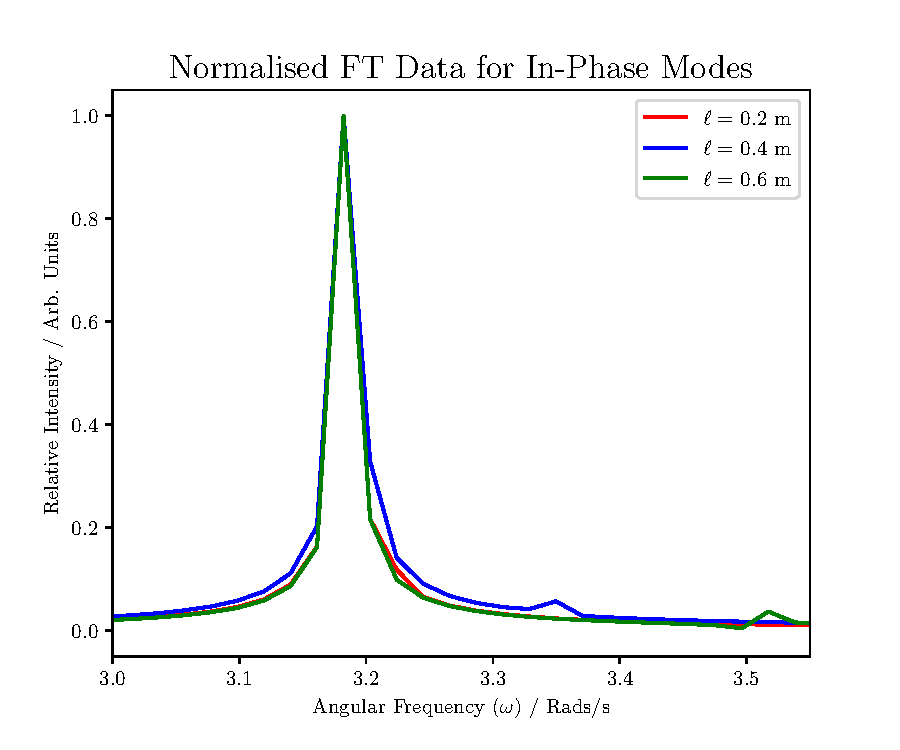
\includegraphics[width = 8 cm]{Normalised In-Phase FT Frequency Comparrison.pdf}
    \caption{In-Phase Fourier Transform Data}
    \label{fig:InPhase}
\end{figure}

A quick $F$ test, again, can reveal no evidence of any dependence on $\ell$. We pool the data from each $\ell$ for a more precise result.

\begin{table}[h]
    \begin{tabular}{@{}lllll@{}}
    \toprule
                            & Rads$/$s    & U ($95 \%$ CI)  & \\ \midrule
    Experimental            & $3.18$      & $0.02$          & \\ 
    Model                   & $3.13$      & $0.00$          & \\ 
    $\textnormal{Model}'$   & $3.19$      & $0.05$          & \\ \bottomrule
    \end{tabular}
 
    \caption{In-Phase Frequency Peaks}
\end{table}

Clearly, our model with experimental data performed significantly more accurately. The model has correctly predicted the lack of any dependence of $ \omega $ on $\ell$ or $k$ in this mode.

\subsection*{Out-of-Phase Mode}

The Out-of-Phase mode is where (according to our model) we should start to expect seeing some dependence of $\omega$ on $k$ and $\ell$.

\begin{table}[h]
\begin{tabular}{llllllllllllllll}
\toprule
                        & $\ell = 0.2$   & $95\%$ CI    & $\ell = 0.4$   & $95\%$ CI    & $\ell = 0.6$   & $95\%$ CI    & \\ \midrule
Experimental            & $3.22$         & $0.02$       & $3.34$         & $0.04$       & $3.52$         & $0.02$       & \\ 
Model                   & $3.17$         & $0.00$       & $3.29$         & $0.01$       & $3.47$         & $0.02$       & \\ 
$\textnormal{Model}'$   & $3.23$         & $0.05$       & $3.34$         & $0.05$       & $3.51$         & $0.05$       & \\ \bottomrule
\end{tabular}
\caption{Out-of-Phase Frequency Peaks}
\end{table}

Note that there is a small peak at around where we experimentally measured $ \omega_n$. The relative intensity of this peak indicates that we haven't got a perfectly out of phase system, but we are quite close.

\begin{figure}[h]
    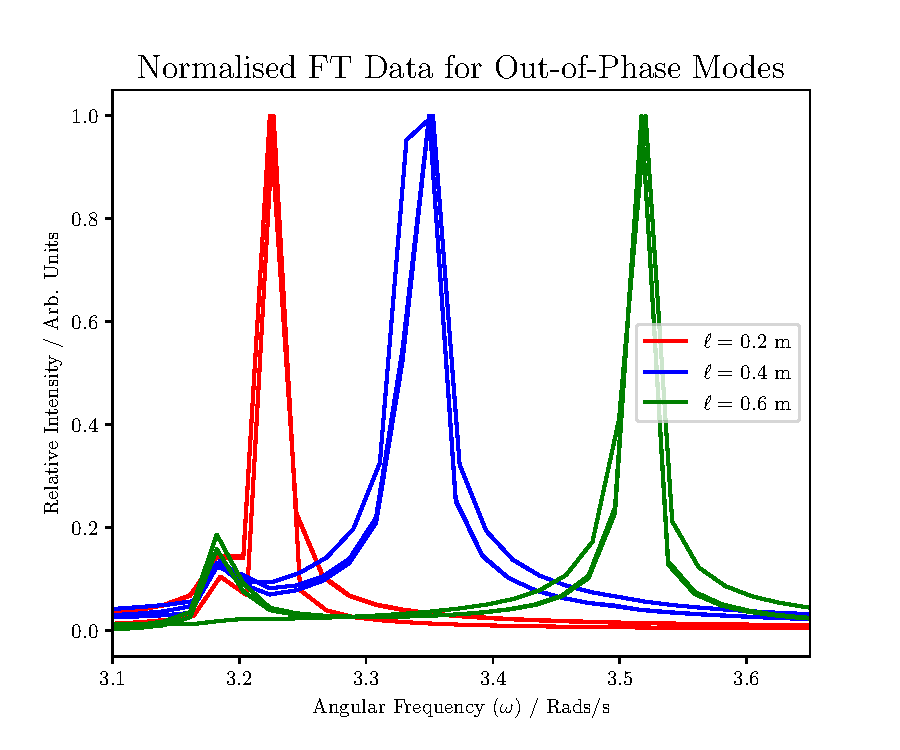
\includegraphics[width = 8 cm]{Normalised Out-of-Phase FT Frequency Comparrison.pdf}
    \caption{Out-of-Phase F.T. Data}
    \label{fig:Out-of-Phase}
\end{figure}

This data again reinforces that our model is capable of predicting the dependence of $\omega$ on $\ell$ and $k$, as well as its inability to make accurate predictions.
\newline
The modified model is significantly more accurate, but less precise. The imprecision of the uncoupled model comes primarily from the initial experimental uncertainty from the first experiment, with uncertainty from the spring constant largely disappearing when added in quadrature.

\subsection*{Beat Mode}

\begin{figure}[h]
    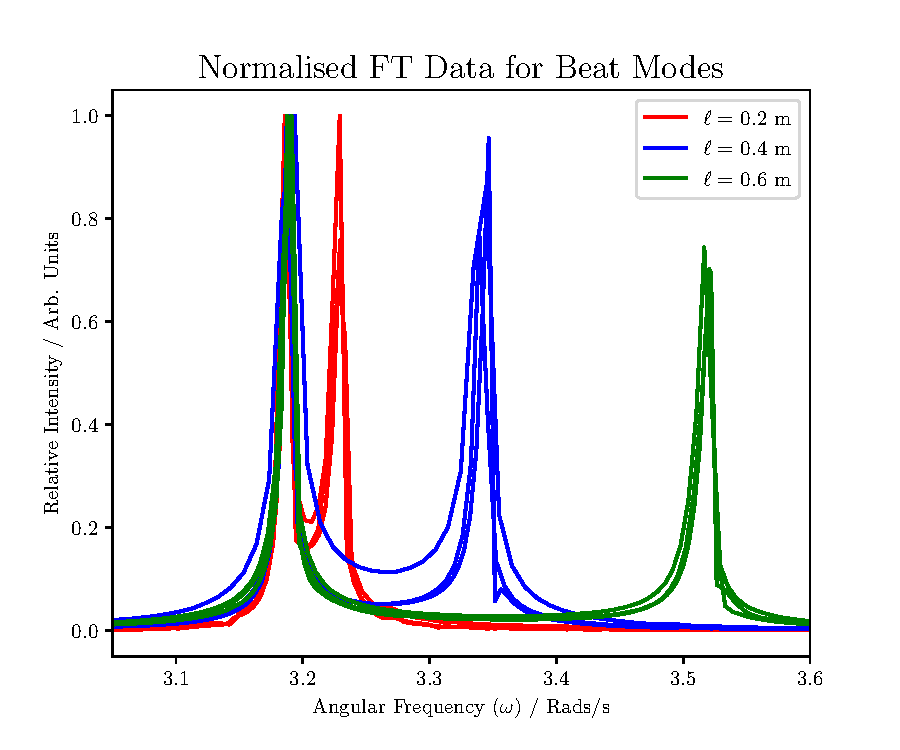
\includegraphics[width = 8 cm]{Normalised Beat FT Frequency Comparrison.pdf}
    \caption{Beat Fourier Transform Data}
    \label{fig:beat}
\end{figure}

The beat mode is expected to have dependance on both $k$ and $\ell$, and be somewhat like an addition of figures \ref{fig:InPhase} and \ref{fig:Out-of-Phase}.

Once again, our model is not capable of precise predictions, but correctly predicts dependancy on certain variables. The model using experimental $\omega_n$ is accurate to within experimental precision

\begin{table}[h]
    \begin{tabular}{llllllllllllllll}
    \toprule
                            & $\ell = 0.2$   & $95\%$ CI    & $\ell = 0.4$   & $95\%$ CI    & $\ell = 0.6$   & $95\%$ CI    & \\ \midrule
    Experimental            & $3.19$         & $0.01$       & $3.19$         & $0.01$       & $3.19$         & $0.01$       & \\ 
    Model                   & $3.13$         & $0.00$       & $3.13$         & $0.00$       & $3.13$         & $0.00$       & \\ 
    $\textnormal{Model}'$   & $3.19$         & $0.05$       & $3.19$         & $0.05$       & $3.19$         & $0.05$       & \\ \bottomrule
    \end{tabular}
    \caption{Beat: First Peak}
\end{table}

\begin{table}[h]
    \begin{tabular}{llllllllllllllll}
    \toprule
                            & $\ell = 0.2$   & $95\%$ CI    & $\ell = 0.4$   & $95\%$ CI    & $\ell = 0.6$   & $95\%$ CI    & \\ \midrule
    Experimental            & $3.23$         & $0.01$       & $3.34$         & $0.01$       & $3.52$         & $0.01$       & \\ 
    Model                   & $3.17$         & $0.00$       & $3.29$         & $0.01$       & $3.47$         & $0.02$       & \\ 
    $\textnormal{Model}'$   & $3.23$         & $0.05$       & $3.34$         & $0.05$       & $3.51$         & $0.05$       & \\ \bottomrule
    \end{tabular}
    \caption{Beat: Second Peak}
\end{table}
        
\section{Numerical Methods}

All of this paper so far has discussed using the small angle approximation to find approximate analytic solutions to the ODE system of equations. We don't need to do this, because we have {\it{computers!}}

Following the excellent instructions found in Prof. Dr. Frank Cichos' \textsc{GitHub} repository\cite{note 2}, we can quite easily create a mathematical model that simulates the pendula. We have the following equations of motions to simulate (the other follows as before):

\begin{equation}
    I \phi_1 = -mgL \sin \left( \phi_1 \right) - k \ell^2 \left( \sin \left( \phi_1 \right) - \sin \left( \phi_2 \right) \right)
\end{equation}

We will run a simulation, perform a Fourier transform on the simulated data and then fit Gaussians to find uncertainties.

We will compare Model, $\textnormal{Model}'$, experimental data and the numerical solutions.

\begin{table}[h]
    \begin{tabular}{lllllllllllllllllll}
    \toprule
                            & $\omega_n$     & U            & $\omega'_0.2$  & U            & $\omega'_0.4$  & U            & $\omega'_0.6$  & U            & \\ \midrule
    Experimental            & $3.19$         & $0.05$       & $3.22$         & $0.02$       & $3.34$         & $0.04$       & $3.52$         & $0.02$       & \\ 
    Model                   & $3.13$         & $0.00$       & $3.17$         & $0.00$       & $3.29$         & $0.01$       & $3.47$         & $0.02$       & \\ 
    $\textnormal{Model}'$   & $3.19$         & $0.05$       & $3.23$         & $0.05$       & $3.34$         & $0.05$       & $3.51$         & $0.05$       & \\
    Numerical               & $3.12$         & $0.01$       & $3.16$         & $0.01$       & $3.27$         & $0.00$       & $3.46$         & $0.00$       & \\ \bottomrule
    \end{tabular}
    \caption{Numerical Methods Comparison}
\end{table}

\begin{figure}[H]
    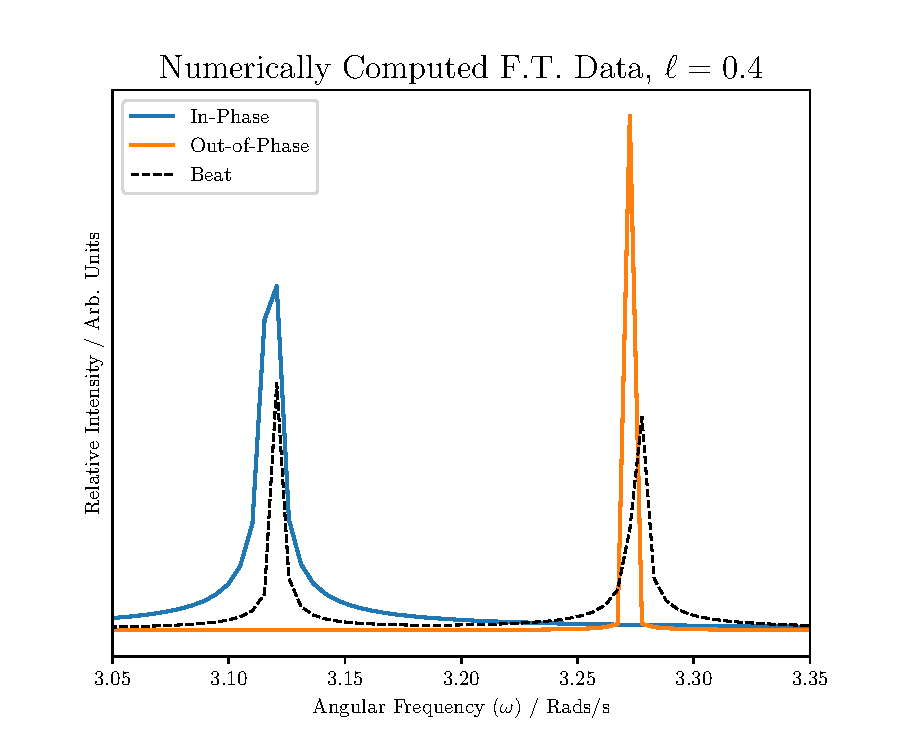
\includegraphics[width = 8 cm]{Numerical.pdf}
    \caption{Beat Fourier Transform Data}
    \label{fig:beat}
\end{figure}

\section{Discussion}

Clearly, our theoretical model by itself is not capable of producing accurate predictions. It is, however, very close to the numerical solution. The proximity of these two models indicates that the small angle approximation does not dramatically decrease the accuracy of the model, and that the inaccuracy of the model comes from other sources.

By inspecting the numerical methods result, we can see that the beat frequency is not quite a perfect superposition of the normal modes. We can exaggerate this by changing the initial angle in the model. This clearly shows the breakdown of the linearity of the ODEs that was initially allowed by the small angle approximation. 

By noting how well the modified model using an experimental $\omega_n$ performs, we can deduce that the original model is failing to account for some core variable in the pendulum. It is likely that this variable is the moment of inertia of the pendula. The assumption that the pendulum is a point mass suspended from a massless string is clearly not correct.

The modified model with experimental $\omega_n$ allows for the most accurate predictions with the least effort. The small angle approximation does not significantly hamper the accuracy of the model. Without the experimental $\omega_n$, the model can make good qualitative predictions but cannot make accurate quantitative ones.

The precision of experimental results has been acceptable; a better measurement of $\omega_n$, likely in the form of a longer experimental trial, could potentially greatly increase the precision of the modified model. The numerical model results can always be improved by more processing time and a smaller time step, but this increase in precision would not be useful, nor would it necessarily be desirable in terms of the computational burden.

Future models could incorporate a more sophisticated expression for the moment of inertia of the pendulum and use strictly theoretical values to make predictions. The numerical method model has not proved significantly more accurate than the analytic small angle approximation model, so it is not necessary to further explore that avenue without significant changes to the system (for example, possibly a larger system of coupled pendula, maybe four or five pendulums all together). 

\pagebreak

\section{Conclusions}

Derived equations of motion using a Taylor series approximation can predict trends and behaviours of the system but cannot offer accurate quantitative predictions. Using an experimentally determined value for $\omega_n$ allows the model to be accurate to within experimental error for minimal additional effort.

The Taylor approximation is very close to the numerical solutions, which suggests that errors in the model stem from assumptions about the pendula's moment of inertia, rather than the small angle approximation.

\section{Acknowledgements}

Prof. Cichos' \textsc{GitHub} repository \cite{GitHub} was very useful, not only because of its explicit recourses for this problem but because of its general educational value. It had some great content regarding Fast-Fourier-Transforms as well.

\vspace*{6pt}

Thank you to those that peer-reviewed my work.

\vspace*{6pt}

All code that I have used, as well as experimental data, diagrams and documentation (including my lab notebook) can be found on the corresponding \textsc{GitHub} repository, accessible \href{https://github.com/Sam-js2/PHYS2113-Lab-Report}{here}.

\begin{thebibliography}{99}

\bibitem{notes} Course notes are available on the \texttt{PHYS2113} Moodle. You can solve the ODEs by making a smart substitution, \textsc{Mathematica} will be happy to help out, and, in in-fact, \textsc{Wolfram Alpha} has a similar coupled pendula system on record.

\vspace*{6pt}

\bibitem{note1} If you haven’t already encountered the Delta function (i.e., have not done \textsc{PHYS2111} yet), $\delta \left( x - a\right) $ is a function (not actually a function) whose value is infinity at $a$ and $0$ elsewhere, and where $ \int_{-\infty}^{\infty} \delta \left( x - a\right)\,dx  = 1$. It is the limit of a Gaussian as $\sigma \to 0$ (this explains the error analysis approach).

\vspace*{6pt}

\bibitem{note 2} From his course at the University of Leipzig, {\it Introduction to Computer Based Modelling}. Titles stack in German. See \cite{GitHub} for the details.

\vspace*{6pt}

\bibitem]{Taylor, JR 2005} J.R. Taylor, 2005, {\it Classical Mechanics}, University Science Books, Virginia USA.

\vspace*{6pt}

\bibitem{GitHub} Cichos, F 2022, {\it Comsoft 2021} Website/Jupyter Notebook, University of Leipzig, Leipzig. \href{https://fcichos.github.io/CompSoft21/course-info/website.html}{Accessed July 2022}, \href{https://github.com/fcichos/CompSoft21}{Source code}.

\end{thebibliography}

\end{document}
